\documentclass[a4paper]{ctexart}
\title{高等代数笔记}
\date{2021.9-2023.2}
\author{陈治华}
\usepackage{amsmath}
\usepackage{amssymb}
\usepackage{graphicx}
\usepackage{subfigure}
\usepackage{tikz}
\usepackage{booktabs}
\begin{document}
\maketitle

\newpage
\tableofcontents
\thispagestyle{empty}
\newpage
\pagenumbering{arabic}

\newpage
\part{线性方程组}
\section{高斯·若尔当算法}
\subsection{线性方程组}
形如下列方程组的方程组被称为线性方程组:
$$
\begin{cases}
a_{11}x_{1}+a_{12}x_{2}+\cdots+a_{1n}x_{n}=b_{1}\\
a_{21}x_{1}+a_{22}x_{2}+\cdots+a_{2n}x_{n}=b_{2}\\
\cdots\\
a_{s1}x_{1}+a_{s2}x_{2}+\cdots+a_{sn}x_{n}=b_{s}\\
\end{cases}
$$

我们在初中学习过二元一次方程组,三元一次方程组的加减消元法与代入消元法,但这两种方法显然在面对一般的线性方程组求解问题时有一些局限,于是我们引入高斯·若尔当算法来求解一般的线性方程组问题。

下面是具体的算法:
首先我们利用第一个方程来去消去其余方程的第一项(在这里我们假设第一个方程的首项系数不是0),方程组会变成这样:

$$
\begin{cases}
a_{11}x_{1}+a_{12}x_{2}+\cdots+a_{1n}x_{n}=b_{1}\\
0+m_{22}x_{2}+\cdots+m_{2n}x_{n}=c_{2}\\
\cdots\\
0+p_{s2}x_{2}+\cdots+p_{sn}x_{n}=c_{s}\\
\end{cases}
$$

这时我们发现,下面s-1个方程也可以被视为一个方程组,不断重复之前的操作,最终方程组会变成这样:

$$
\begin{cases}
a_{11}x_{1}+a_{12}x_{2}+\cdots+a_{1n}x_{n}=b_{1}\\
0+m_{22}x_{2}+\cdots+m_{2n}x_{n}=c_{2}\\
\cdots\\
0+0+\cdots+t_{sn}x_{n}=t_{s}\\
\end{cases}
$$

直观上看就像楼梯一样,我们称之为阶梯形。方程组变形到这一步以后,我们就可以讨论方程组解的可能性了。但是我们暂且不提,为了后续研究的方便,我们引入矩阵的概念。

\subsection{矩阵与线性方程组的解}
我们继续考虑开头提出的方程组:

$$
\begin{cases}
a_{11}x_{1}+a_{12}x_{2}+\cdots+a_{1n}x_{n}=b_{1}\\
a_{21}x_{1}+a_{22}x_{2}+\cdots+a_{2n}x_{n}=b_{2}\\
\cdots\\
a_{s1}x_{1}+a_{s2}x_{2}+\cdots+a_{sn}x_{n}=b_{s}\\
\end{cases}
$$

我们发现在运算的过程中,我们只是对于方程的系数与常数项进行了运算,未知数本身并没有参与任何运算。那么我们对于一个方程组就可以只写出它的系数与常数项,把它们放在应该在的位置上,组成一张举行的表,这张表被称为方程组的增广矩阵。如果只用系数来进行列表,那么我们就称这张表为系数矩阵。比如上述方程组的增广矩阵与系数矩阵为:

$$
\begin{pmatrix}
a_{11}&a_{12}&\cdots&a_{1n}&b_{1}\\
a_{21}&a_{22}&\cdots&a_{2n}&b_{2}\\
\vdots&\vdots&\ddots&\vdots&\vdots\\
a_{s1}&a_{s2}&\cdots&a_{sn}&b_{s}\\
\end{pmatrix}
$$

$$
\begin{pmatrix}
a_{11}&a_{12}&\cdots&a_{1n}\\
a_{21}&a_{22}&\cdots&a_{2n}\\
\vdots&\vdots&\ddots&\vdots\\
a_{s1}&a_{s2}&\cdots&a_{sn}\\
\end{pmatrix}
$$

\textbf{定义:由s·m个数排成的s行,m列的一张表被称为一个s·m矩阵,其中的每一个数被称为矩阵的一个元素,第i行与第j列交叉的元素被称为(i,j)元。}

矩阵通常用大写的英文字母A,B,C···来表示。元素全为0的矩阵被称为\textbf{零矩阵},简记为0;如果一个矩阵的行数与列数相等,则称它为方阵,m行m列的矩阵也可以被称为m阶矩阵或m级矩阵。

我们现在就展示利用高斯·若尔当算法,结合矩阵来解线性方程组的过程:

$$
\begin{cases}
x_{1}+3x_{2}+x_{3}+2x_{4}=4\\
3x_{1}+4x_{2}+2x_{3}-3x_{4}=6\\
-x_{1}-5x_{2}+4x_{3}+x_{4}=11\\
2x_{1}+7x_{2}+x_{3}-6x_{4}=-5\\
\end{cases}
$$

写出它对应的增广矩阵:

$$
\begin{pmatrix}
1&3&1&2&4\\
3&4&2&-3&6\\
-1&-5&4&1&11\\
2&7&1&-6&-5\\
\end{pmatrix}
$$

我们现在就可以运用矩阵的第一行来消去矩阵后三行的第一个元素,得到一个新的矩阵。(用下面三行来消也无伤大雅,这不是重点。)\textbf{注意:这个矩阵与之前的矩阵绝对不是相同的矩阵!只是这两个矩阵对应的线性方程组同解而已。至于这两个矩阵间更加具体的关系,我们放在以后的章节来讨论。}

$$
\begin{pmatrix}
1&3&1&2&4\\
0&-5&-1&-9&-6\\
0&-2&5&3&15\\
0&-3&9&-4&17\\
\end{pmatrix}
$$

重复这种操作,我们来消去最下面两行的第二列数字:

$$
\begin{pmatrix}
1&3&1&2&4\\
0&-5&-1&-9&-6\\
0&1&-4&7&-2\\
0&-3&9&-4&17\\
\end{pmatrix}
$$

$$
\begin{pmatrix}
1&3&1&2&4\\
0&0&-21&26&-16\\
0&1&-4&7&-2\\
0&0&-3&17&11\\
\end{pmatrix}
$$

我们把顺序调整一下,从而让我们看的更加舒服。

$$
\begin{pmatrix}
1&3&1&2&4\\
0&1&-4&7&-2\\
0&0&-21&26&-16\\
0&0&-3&17&11\\
\end{pmatrix}
$$

下面我们来进行最后的消元。

$$
\begin{pmatrix}
1&3&1&2&4\\
0&1&-4&7&-2\\
0&0&-21&26&-16\\
0&0&0&93&93\\
\end{pmatrix}
$$

到这里我们已经可以通过从最后一行向前逆向得到方程组的解了,但我们不妨将其化简成为\textbf{最简阶梯形}。

$$
\begin{pmatrix}
1&0&0&0&3\\
0&1&0&0&-1\\
0&0&1&0&2\\
0&0&0&1&1\\
\end{pmatrix}
$$

于是我们就可以得到原方程组的解了:

$$
\begin{cases}
x_{1}=3\\
x_{2}=-1\\
x_{3}=2\\
x_{4}=1\\
\end{cases}
$$

我们也可以写成列向量的形式:

$$
\left(
\begin{array}{cccc}
 x_{1}\\
 x_{2}\\
 x_{3}\\
 x_{4}\\
\end{array}
\right )
=
\left(
\begin{array}{cccc}
3\\
-1\\
2 \\
1\\
\end{array}
\right )
$$

至于为什么写成列向量而不是行向量,我们则会在后文讨论矩阵的运算法则的时候给出解答。

\section{线性方程组解的情况与判定准则}
\subsection{线性方程组解的情况}
线性方程组的解可能有唯一解,无穷解,也可能没有解(比如出现了0=1的矛盾方程)。

我们设系数矩阵化为阶梯形之后的非零行数为r,增广矩阵化为阶梯形之后的非零行数为d。显然,若r=d=n,那么方程组具有唯一的解;若r<d,那么方程组无解(r不会大于d);若r=d<n,那么方程组有无穷解。\textbf{(事实上我们知道:设方程组通解构成的空间为V,则dimV=n-r,我们就可以知道解空间的维度了。)}从几何上我们很容易知道d不会大于n,所以我们没有必要讨论d>n的可能性。

\subsection{矩阵的秩}
一个矩阵通过行变换化为阶梯形以后,有r个非零行,那么矩阵的秩就是r。如果矩阵是A,那么我们常把矩阵的秩记为rankA。这种定义下的秩我们称之为矩阵的行秩,对称的,我们也可以定义矩阵的列秩。于是我们很自然的想到这个问题:

\textit{如何证明矩阵的行秩与列秩相等?}

想解决这个问题,我们就要从向量的角度来重新认识矩阵了。我们暂且按下不表,就默认矩阵的行秩等于列秩吧。

\subsection{线性方程组解的情况的判定准则}
设n元线性方程组的系数矩阵为A,n元线性方程组的增广矩阵为B:

\textit{若rankA=rankB=n,那么原方程组有唯一一组解}

\textit{若rankA=rankB<n,那么原方程组有无穷组解}

\textit{若rankA<rankB,那么原方程组无解}

在这里我们补充定义一种特殊的线性方程组,我们就可以利用上述准则得到一些有价值的推论了。

定义,在线性方程组中,如果所有常数项为零,我们就成这个线性方程组是\textbf{齐次线性方程组}。

$$
\begin{cases}
a_{11}x_{1}+a_{12}x_{2}+\cdots+a_{1n}x_{n}=0\\
a_{21}x_{1}+a_{22}x_{2}+\cdots+a_{2n}x_{n}=0\\
\cdots\\
a_{s1}x_{1}+a_{s2}x_{2}+\cdots+a_{sn}x_{n}=0\\
\end{cases}
$$

对于这种方程组的解,我们只要考察它的系数矩阵即可。

显然,这个方程组有\textbf{零解};若rankA<n,那么这个方程就会有其他的\textbf{非零解}。同时我们发现了两个推论:

\textit{推论1:若齐次线性方程组有一个非零解,那么这个方程组一定有无穷组解。}

\textit{推论2:m个n元一次方程组成的齐次线性方程组,若m<n,那么方程组一定有无穷组解。}

\subsection{练习题}

一个投资者想把一万元投资给三个企业,A1,A2,A3,所得的利润率分别为12$\%$,15$\%$,22$\%$。如果他投给A3的钱等于投给A1,A2的钱的和,求总利润S(单位:千元)的最大值与最小值。并求此时分别给三家企业投资了多少元?

解:设投资者给这三家企业分别投资了$x_{1},x_{2},x_{3}$元。根据题意我们可以得到方程组:

$$
\begin{cases}
x_{1}+x_{2}+x_{3}=10\\
-x_{1}-x_{2}+x_{ 3}=0\\
\end{cases}
$$

于是我们的得到:

$$
\begin{cases}
x_{3}=5\\
x_{1}+x_{2}=5\\
\end{cases}
$$

于是我们可以列出利润的表达式:

$$
\begin{aligned}
S&=1.12x_{1}+1.15x_{2}+1.22x_{3}\\
  &=1.12x_{1}+1.15(5-x_{1})+6.1\\
  &=-0.03x_{1}+11.85\\
\end{aligned}
$$

 于是我们很容易知道S的最大值为11.85(千元),此时$x_{1}=0,x_{2}=x_{3}=5$,即给A1公司投资零元,给A2,A3公司投资5千元;
 S的最小值为11.7(千元),此时$x_{1}=x_{3}=5,x_{2}=0$,及给A2公司投资零元,给A1,A3公司投资5千元。
 
\section{数域}
我们知道数学中存在着许许多多的结构,拓扑结构,序结构等。代数上同样也会有精巧的代数结构,比如群,环,域等。对于它们具体的讨论我们需要放到后续的《抽象代数》的学习中,在这里,我们只简要介绍最简单的一种域——数域。

\subsection{数域的概念}
\textbf{定义:设F是一个含有0,1的数集,对加减乘除四则运算封闭,那么称系统(F;+,-,$\times$,$\div$)是一个数域。}

例如,我们熟知的有理数,实数,复数都是数域。

\textit{证明最小的数域是有理数域。}

\textit{证明:首先证明数域一定包含全体有理数。F包含0,1,并且对于加减保持封闭,于是我们就得到了全体整数。F又对除法保持封闭,那么我们就得到了全体的有理数。}

\textit{再证全体有理数构成一个数域。设任意两个有理数(已经化为既约形式)$\frac{a}{b}$,$\frac{c}{d}$。我们考虑它们的四则运算:}

$$
\frac{a}{b}+\frac{c}{d}=\frac{ad+bc}{bd}\\
$$

$$
\frac{a}{b}-\frac{c}{d}=\frac{ad-bc}{bd}\\
$$

$$
\frac{a}{b}\times\frac{c}{d}=\frac{ac}{bd}\\
$$

$$
\frac{a}{b}\div\frac{c}{d}=\frac{ad}{bc}\\
$$

\textit{显然,它们运算的结果也都是有理数,即有理数集对于加减乘除的运算是封闭的,它确实是一个数域。}

\textit{于是我们证明了最小的数域是有理数域。}

我们于是得到一个结论与一个推论:

\textbf{有理数域是最小的数域。}

我们在证明上述结论的过程中发现,任何数域,都可以构造出全体有理数,于是我们得到推论:

\textbf{任何数域必然包含有理数域。}

\subsection{数域的构造}
我们已经知道了数域的定义,那么我们是否可以根据要求构造出我们需要的数域呢?

我们已知:\textbf{任何数域都必然包含有理数域。}

\textit{请构造出包含$\sqrt{2}$的最小数域。}

\textit{解:我们首先构造出一个包含$\sqrt{2}$的数域。}

\textit{我们知道属于肯定包含有理数域,在此基础上还需要包含$\sqrt{2}$,所以我们不妨假设数域可以表示为:}

$$
F=\{a+b\sqrt{2}\mid a、b\in\mathbb{Q} \}
$$

\textit{如果这个集合可以构成数域,那么这就是我们求的最小数域。(因为我们在用必要条件进行构造。)取集合中的两个元素进行四则运算:}

$$
(a+b\sqrt{2})+(c+d\sqrt{2})=(a+c)+(b+d)\sqrt{2}
$$

$$
(a+b\sqrt{2})-(c+d\sqrt{2})=(a-c)+(b-d)\sqrt{2}
$$

$$
(a+b\sqrt{2})\times(c+d\sqrt{2})=(ac+2bd)+(ad+bc)\sqrt{2}
$$

$$
(a+b\sqrt{2})\div(c+d\sqrt{2})=\frac{a+b\sqrt{2}}{c+d\sqrt{2}}=\frac{(a+b\sqrt{2})\times(c-d\sqrt{2})}{(c+d\sqrt{2})\times(c-d\sqrt{2})}=\frac{ac-2bd}{c^2-2d^2}+\frac{bc-ad}{c^2-2d^2}\sqrt{2}
$$

\textit{我们发现,我们构造的集合对于四则运算是封闭的,的确是一个数域。所以我们得到了包含$\sqrt{2}$的最小数域F。}

\section{附录:线性方程组的两种视角}
在这一个章节,我们来讨论线性方程组的两个视角,以二元一次方程组与三元一次方程组为例。


我们考虑这样一个方程组:
$$
\begin{cases}
3x-2y=-1\\
x-y=-1\\
\end{cases}
$$

其中每一行都是一个二元一次方程,都代表着平面上的一条直线,我们可以在坐标系中绘制出来:

\begin{figure}[htp]
\centering
\begin{tikzpicture}
\draw [->](-4,0)--(4,0)node[right]{$x$};
\draw [->](0,-4)--(0,4)node[right]{$y$};
\node at (-0.2,-0.2) {$O$};
\draw [domain=-2:2,samples=1000,thick] plot(\x,{0.5+1.5*\x});
\draw [domain=-3:3,samples=1000,thick] plot(\x,{1+\x});
\node at(1.5,2.2){$P$};
\draw[dashed](1,2)--(1,0);
\draw[dashed](1,2)--(0,2);
\foreach \x in {-3,-2,-1,1,2,3} {\draw (\x,0)node[below]{$\x$}--(\x,.1);}
\foreach \y in {-3,-2,-1,1,2,3} {\draw (0,\y)node[left]{$\y$}--(-.1,\y);}
\end{tikzpicture}
\caption{行视角}
\end{figure}

如图所示,两条直线的交点,就对应着原方程组的解。

同时,我们也可以换一种角度来看待这个方程组:

$$
\begin{cases}
3x-2y=-1\\
x-y=-1\\
\end{cases}
$$

我们可以沿着列的方向来看待它,于是原方程化为:

$$
\left(
\begin{array}{cccc}
 3\\
 1\\
\end{array}
\right )x
+
\left(
\begin{array}{cccc}
 -2\\
 -1\\
\end{array}
\right )y
=
\left(
\begin{array}{cccc}
-1\\
-1\\
\end{array}
\right )
$$

于是问题转化为,求解目标向量沿着两个基向量方向分解得到的坐标。虽然这本身仍然是一个困难的问题,但是这种观点会为我们以后的研究提供方便。

\begin{figure}[htp]
\centering
\begin{tikzpicture}
\draw [->](-4,0)--(4,0)node[right]{$x$};
\draw [->](0,-4)--(0,4)node[right]{$y$};
\node at (-0.2,-0.2) {$O$};
\draw[->,thick](0,0)--(3,1)node[right]{$\alpha$};
\draw[->,thick](0,0)--(-2,-1)node[right]{$\beta$};
\draw[->,thick](0,0)--(-1,-1)node[right]{$\gamma$};
\draw[dashed](3,1)--(-1,-1);
\draw[dashed](-1,-1)--(-4,-2);
\draw[dashed](-2,-1)--(-4,-2)node[left]{$2\beta$};
\foreach \x in {-3,-2,-1,1,2,3} {\draw (\x,0)node[below]{$\x$}--(\x,.1);}
\foreach \y in {-3,-2,-1,1,2,3} {\draw (0,\y)node[left]{$\y$}--(-.1,\y);}
\end{tikzpicture}
\caption{列视角}
\end{figure}

\section{附录:线性方程组的解的结构}
我们现在开始研究,一般的线性方程组解的结构:

现在有方程组如下:
$$
\begin{cases}
a_{11}x_{1}+a_{12}x_{2}+\cdots+a_{1n}x_{n}=b_{1}\\
a_{21}x_{1}+a_{22}x_{2}+\cdots+a_{2n}x_{n}=b_{2}\\
\cdots\\
a_{m1}x_{1}+a_{m2}x_{2}+\cdots+a_{mn}x_{n}=b_{m}\\
\end{cases}
$$

我们写出其增广矩阵:
$$
\begin{pmatrix}
a_{11}&a_{12}&\cdots&a_{1n}&b_{1}\\
a_{21}&a_{22}&\cdots&a_{2n}&b_{2}\\
\vdots&\vdots&\ddots&\vdots&\vdots\\
a_{m1}&a_{m2}&\cdots&a_{mn}&b_{m}\\
\end{pmatrix}
$$

利用高斯·若尔当算法将其化为阶梯形矩阵以后为:
$$
\setcounter{MaxMatrixCols}{20}
\begin{pmatrix}
b_{11}&b_{12}&\cdots&0&\cdots&0&\cdots&0&\cdots&b_{1n}&c_{1}\\
&&&b_{2j_{j2}}&\cdots&0&\cdots&0&\cdots&b_{2n}&c_{2}\\
&&&&&b_{3j_{j3}}&\cdots&0&\cdots&b_{3n}&c_{3}\\
&&&&&&\cdots&\cdots&\cdots&\cdots&\cdots\\
&&&&&&&b_{rj_{r}}&\cdots&b_{rn}&c_{r}\\
&&&&&&&&&&\vdots\\
&&&&&&&&&&c_{m}\\
\end{pmatrix}
$$

若$c_{r+i}\neq 0 (i=1,2,\cdots,m-r)$,那么显然原方程组无解(出现了0=1这种矛盾方程)。(此时增广矩阵的秩大于系数矩阵的秩,我们之前得到的结论仍然成立。)

如果$c_{r+i}= 0 (i=1,2,\cdots,m-r)$,同时我们有$r=n$,那么此时我们从下向上可以得到方程组的唯一一组解,也没有什么结构可言。

如果$r<n$(显然r不会比n大),那么我们就会得到一些未定元素(准确地说是n-r个)(因为只有规定n-r个未定元,才能从下向上接出方程组)。

最终我们得到的方程组的解会具有以下的形式:

$$
\left(
\begin{array}{c}
  x_{1}\\
  x_{2}\\
  \vdots\\
  x_{r}\\
  x_{r+1}\\
  x_{r+2}\\
  \vdots\\
  x_{n}\\
\end{array}
\right)
=
\left(
\begin{array}{c}
  d_{1}\\
  d_{2}\\
  \vdots\\
  d_{r}\\
  0\\
  0\\
  \vdots\\
  0\\
\end{array}
\right)
+
\left(
\begin{array}{c}
  -e_{1,r+1}\\
  -e_{2,r+1}\\
  \vdots\\
  -e_{r,r+1}\\
  1\\
  0\\
  \vdots\\
  0\\
\end{array}
\right)
t_{1}
+
\left(
\begin{array}{c}
  -e_{1,r+2}\\
  -e_{2,r+2}\\
  \vdots\\
  -e_{r,r+2}\\
  0\\
  1\\
  \vdots\\
  0\\
\end{array}
\right)
t_{2}
+
\cdots
+
\left(
\begin{array}{c}
  -e_{1,n}\\
  -e_{2,n}\\
  \vdots\\
  -e_{r,n}\\
  0\\
  0\\
  \vdots\\
  1\\
\end{array}
\right)
t_{n-r}
$$

其中:$r_{1},r_{2},\cdots,r_{n-r} \in \mit{F}$,表示我们讨论的所在数域。

这便是线性方程组向量形式的通解了。

\part{向量与矩阵}
\section{向量空间}
\subsection{实数与复数}
一个复数是一个有序对(a,b),其中$a,b\in\mathbb{R}$,我们可以把它写成代数形式为a+bi。其中$i^2=-1$。

同时复数也有三角形式:$r(cos\theta+isin\theta)$,以及指数形式:$re^{i\theta}$。其中$r=\sqrt{a^2+b^2}$。

复数运算的几何意义如图所示:
\begin{figure}[htp]
\centering
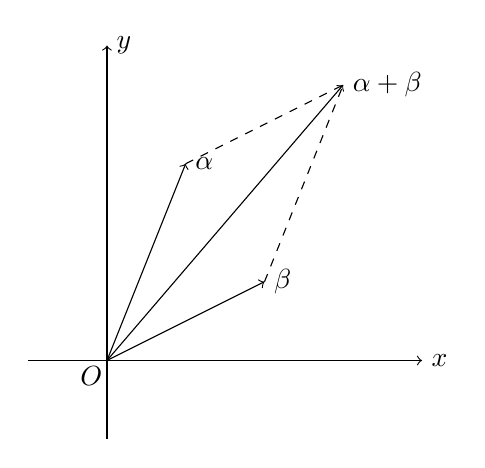
\begin{tikzpicture}
\draw [->](-1,0)--(4,0)node[right]{$x$};
\draw [->](0,-1)--(0,4)node[right]{$y$};
\node at (-0.2,-0.2) {$O$};
\draw[->](0,0)--(1,2.5)node[right]{$\alpha$};
\draw[->](0,0)--(2,1)node[right]{$\beta$};
\draw[->](0,0)--(3,3.5)node[right]{$\alpha + \beta$};
\draw[dashed](1,2.5)--(3,3.5);
\draw[dashed](2,1)--(3,3.5);
\end{tikzpicture}
\caption{复数的加法}
\end{figure}

\begin{figure}[htp]
\centering
\begin{tikzpicture}
\draw [->](-1,0)--(4,0)node[right]{$x$};
\draw [->](0,-1)--(0,6)node[right]{$y$};
\node at (-0.2,-0.2) {$O$};
\draw[->](0,0)--(1,2.5)node[right]{$\alpha$};
\draw[->](0,0)--(2,1)node[right]{$\beta$};
\draw[->](0,0)--(-0.5,6)node[left]{$\alpha \cdot \beta$};
\draw[dashed](1,0)--(2,1);
\draw[dashed](1,2.5)--(-0.5,6);
\end{tikzpicture}
\caption{复数的乘法}
\end{figure}

我们发现复数的加法即为向量的加法,遵循平行四边形定则。复数的乘法则是向量的旋转同时伴有放缩,即辐角相加,模长相乘。我们给出一个简短的证明:

\textit{
证明:设两个复数分别为$r_1(cos\theta_1+isin\theta_1)$,$r_2(cos\theta_2+isin\theta_2)$。
于是我们根据复数的计算法则有:}
$$
\alpha \cdot \beta = r_1 r_2 (cos\theta_1 cos\theta_2 -sin\theta_1 sin\theta_2 +i(sin\theta_1 cos\theta_2 +cos\theta_1 sin\theta_2))
$$
$$
\alpha \cdot \beta = r_1 r_2(cos(\theta_1+\theta_2)+isin(\theta_1+\theta_2))
$$

复数的基础知识就介绍到这里,关于复数的其他知识我们放到以后再进行介绍。(by the way: 我们会在不太远的后文证明,每一个复数都等价于一个矩阵,到那时或许你就会对于复数和矩阵有更深刻的理解。)

\subsection{几何向量}
平面向量的相关知识因为在中学中已经学过,所以我们直接对空间向量进行简要提及。
与平面向量类似,空间向量的加法同样满足平行四边形法则:

同样的,平面向量的那些运算可以平行推广到空间向量,这里就不加赘述了。

于是我们很自然地想到下一个问题,就是三维以上,还有向量的概念么?会是什么样的呢?

\begin{figure}[htp]
\centering
\begin{tikzpicture}
\draw [->](-1,0,0)--(4,0,0)node[right]{$x$};
\draw [->](0,-1,0)--(0,4,0)node[right]{$y$};
\draw [->](0,0,-1)--(0,0,4)node[right]{$z$};
\node at (-0.2,-0.2,-0.2) {$O$};
\draw[->](0,0,0)--(1,2.5,2)node[right]{$\alpha$};
\draw[->](0,0,0)--(2,1,-1)node[right]{$\beta$};
\draw[->](0,0,0)--(3,3.5,1)node[right]{$\alpha + \beta$};
\draw[dashed](1,2.5,2)--(3,3.5,1);
\draw[dashed](2,1,-1)--(3,3.5,1);
\end{tikzpicture}
\caption{空间向量的表示}
\end{figure}

\subsection{数组向量}
我们对于更高维度的向量,用几何方法已经不方便表示了,于是我们开始讨论数组向量。我们首先给出n维向量空间与n维数组向量的定义:

\textit{数域K上所有n元有序数组组成的集合$K^n$,连同定义在它上面的加法与数乘运算及其满足的八条运算律一起,称为数域K上的一个\textbf{n维向量空间},这个向量空间的每一个元素都被称为n维向量,一般写为$\alpha =(a_1,a_2,\cdots,a_n)$,称$a_i$为$\alpha$的第i个分量。}

\textit{加法与数乘的定义:}

\textit{$(a_1,a_2,\cdots,a_n)+(b_1,b_2,\cdots,b_n)=(a_1+b_1,a_2+b_2,\cdots,a_n+b_n)$}

\textit{$k(a_1,a_2,\cdots,a_n)=(ka_1,ka_2,\cdots,ka_n)$}

\textit{八条运算律如下:}

\begin{itemize}
\item \textit{$\alpha+\beta=\beta+\alpha$ (加法交换律)}
\item \textit{$(\alpha+\beta)+\gamma=\beta+(\alpha+\gamma)$ (加法结合律)}
\item \textit{存在零元素,使得:$0+\alpha=\alpha+0=\alpha$}
\item \textit{存在负元素,使得:$\alpha + (-\alpha)=(-\alpha)+\alpha=0$}
\item \textit{$1\alpha=\alpha$}
\item \textit{$(kl)\alpha=k(l\alpha)$}
\item \textit{$(k+l)\alpha=k\alpha+l\alpha$}
\item \textit{$k(\alpha +\beta)=k\alpha +k\beta$}
\end{itemize}

我们很容易发现,平面与空间向量都是满足以上定义的。
事实上,我们可以忘记加法与数乘的定义,仅仅将其视为两种特定的运算,我们给出了一般线性空间的定义。即具有加法与数乘结构的满足以上八条算律的空间被称为线性空间,或向量空间。

\textit{例:数域F上所有的一元多项式,对于多项式的加法以及数对多项式的乘法满足以上八条算律,那么它们也构成一个线性空间,其中的每个元素(多项式)也可以被称为是这个线性空间的向量。}

于是我们发现,各种线性空间与数组线性空间在抽象性质上具有一致性,换言之,我们解决数组向量空间中的问题,就顺带着解决了一切线性空间的问题(因为存在着一一映射,从其他线性空间映射到数组向量空间)。这就是代数的特点——对于结构进行细致的研究,得到适用于各种空间的结论。

我们介绍几个线性空间的基本性质:

\begin{itemize}
\item \textit{零向量具有唯一性}
\item \textit{负向量具有唯一性}
\item \textit{$0\alpha=0,k 0=0, (-1)\alpha=-\alpha$}
\item \textit{若$k\alpha=0$,则$k=0$或$\alpha=0$。}
\end{itemize}

\textit{证明:(1):$0_1+0_2=0_1=0_2+0_1=0_1$}

\textit{(2):$\beta =\beta+0=\beta +\alpha +\gamma=\gamma$}

\textit{(3):$\alpha+0\alpha=(1+0)\alpha=\alpha$,于是$\alpha+0\alpha+(-\alpha)=0\alpha=0$}

\textit{$(-1)\alpha=\alpha+(-\alpha)+(-1)\alpha=-\alpha$}

\textit{$k0=k(\alpha+(-\alpha))=k\alpha+k(-1)\alpha=0\alpha=0$}

\textit{(4)若k不为零,则$\alpha=k^{-1}(k\alpha)=0$}

这几条性质对于我们所熟悉的二维,三维向量空间是十分平凡的,我们在这里只是纯粹用代数的知识再证明了一遍罢了。

\subsection{向量的线性相关性}
下面我们来讨论向量的线性相关性,我们先举两个例子,从几何层面上感性认识,如下图所示:

\begin{figure}[htp]
\centering
\begin{tikzpicture}
\draw [->](-4,0)--(4,0)node[right]{$x$};
\draw [->](0,-4)--(0,4)node[right]{$y$};
\node at (-0.2,-0.2) {$O$};
\draw[->](0,0)--(1,2.5)node[right]{$\alpha$};
\draw[->](0,0)--(2,1)node[right]{$\beta$};
\draw[->](0,0)--(-3,-3.5)node[right]{$\gamma=-(\alpha+\beta)$};
\draw[dashed](-3,-3.5)--(-2,-1)node[left]{$\alpha$};
\draw[dashed](-2,-1)--(0,0)node[right]{$\beta$};
\end{tikzpicture}
\caption{线性相关}
\end{figure}

如图所示,我们说向量$\alpha \beta \gamma$线性相关,即为我们可以用$\alpha \beta \gamma$的一个非零线性组合得到零向量。比如这里的$\alpha+\beta+\gamma=0$。

类似的,我们给出一个线性无关的例子:

\begin{figure}[htp]
\centering
\begin{tikzpicture}
\draw [->](-1,0,0)--(4,0,0)node[right]{$x$};
\draw [->](0,-1,0)--(0,4,0)node[right]{$y$};
\draw [->](0,0,-1)--(0,0,4)node[right]{$z$};
\node at (-0.2,-0.2,-0.2) {$O$};
\draw[->](0,0,0)--(3,0,3.5)node[right]{$\alpha$};
\draw[->](0,0,0)--(0,3,-1)node[right]{$\beta$};
\draw[->](0,0,0)--(3,1.5,2)node[right]{$\gamma$};
\end{tikzpicture}
\caption{线性无关}
\end{figure}

$k_1\alpha+k_2\beta+k_3\gamma=0$当且仅当$k_1=k_2=k_3=0$时成立。
换言之,这三个向量之间不存在互相表示的关系。

下面,我们给向量组的线性相关给出一个一般的定义:

\textit{定义:对于向量组$\alpha_1,\alpha_2,\cdots,\alpha_n$,如果方程$\lambda_1\alpha_1+\lambda_2\alpha_2+\cdots+\lambda_n\alpha_n=0$有一组非零解,那么我们称这个向量组线性相关,反之称为线性无关。}

我们设每个向量具有以下形式:

$$
\alpha_i=
\left(
\begin{array}{cccc}
a_{i1}\\
a_{i2}\\
\cdots \\
a_{is}\\
\end{array}
\right )
$$

那么方程组就可以变成:
$$
\begin{cases}
a_{11}\lambda_{1}+a_{21}\lambda_{2}+\cdots+a_{n1}\lambda_{n}=0\\
a_{12}\lambda_{1}+a_{22}\lambda_{2}+\cdots+a_{n2}\lambda_{n}=0\\
\cdots\\
a_{1s}\lambda_{1}+a_{2s}\lambda_{2}+\cdots+a_{ns}\lambda_{n}=0\\
\end{cases}
$$

故我们只需要考虑以下矩阵的秩即可:
$$
\begin{pmatrix}
a_{11}&a_{21}&\cdots&a_{n1}\\
a_{12}&a_{22}&\cdots&a_{n2}\\
\vdots&\vdots&\ddots&\vdots\\
a_{1s}&a_{2s}&\cdots&a_{ns}\\
\end{pmatrix}
$$

这就是第一章讨论的内容了。下面我们引入一个新的概念:极大线性无关组。

\textit{我们考虑这样一个向量组:$\{\alpha_1,\alpha_2,\cdots,\alpha_n\}$,如果我们他们可以被其中i个向量线性表出(不妨设这i个向量为$\{\alpha_1,\alpha_2,\cdots,\alpha_i\}$),并且这i个向量彼此线性无关,那么就称这i个向量构成的向量组是原向量组的一个极大线性无关组。}

一个例子如下图所示:

\begin{figure}[htp]
  \centering
  \begin{tikzpicture}
    \draw[->](0,0)--(3,1)node[right]{$\alpha$};
    \draw[->](0,0)--(1,2)node[right]{$\beta$};
    \draw[->](0,0)--(-2,-3)node[right]{$\gamma$};
    \draw[->](0,0)--(-1.5,2.5)node[right]{$\omega$};
  \end{tikzpicture}
  \caption{极大线性无关组}
\end{figure}

其中:

$$
\alpha=
\left(
  \begin{array}{cccc}
    3\\
    1\\
  \end{array}
\right)
,
\beta=
\left(
  \begin{array}{cccc}
    1\\
    2\\
  \end{array}
\right)
,
\gamma=
\left(
  \begin{array}{cccc}
    -2\\
    -3\\
  \end{array}
\right)
,
\omega=
\left(
  \begin{array}{cccc}
    -1.5\\
    2.5\\
  \end{array}
\right)
$$

我们先证明$\alpha$与$\beta$是线性无关的:

$$
k_1\alpha+k_2\beta
=
\left(
  \begin{array}{cccc}
    3k_1+1k_2\\
    1k_1+2k_2\\
  \end{array}
\right)
=
0
$$
  
显然,等式成立当且仅当:

$$
k_1=k_2=0
$$

于是$\alpha$,$\beta$线性无关。

同时,我们容易发现:

$$
-\frac{1}{5}\alpha-\frac{7}{5}\beta=\gamma
$$

$$
-\frac{11}{10}\alpha+\frac{9}{5}\beta=\omega
$$

也就是说,向量组中的其他向量的确可以被$\alpha$,$\beta$线性表出,所以它们构成这个向量组的一个极大线性无关组。

同样的,$\gamma$,$\omega$也构成一个极大线性无关组,也就是说,极大线性无关组可以有很多种。

下面我们来进一步讨论更一般的极大线性无关组的相关性质:

\textit{向量组$\{\alpha_1,\alpha_2,\cdots,\alpha_n\}$线性相关的充要条件是,其中至少有一个向量可以被其他向量线性表出。}

证明:我们假设向量$\alpha_{i}$可以被其他向量线性表出,那么可以写为:

$$
\alpha_{i}=k_{1}\alpha_{1}+k_{2}\alpha_{2}+\cdots+k_{n-1}\alpha_{n}
$$

于是我们就可以得到:
$$
k_{1}\alpha_{1}+k_{2}\alpha_{2}+\cdots+k_{n-1}\alpha_{n}+(-1)\alpha_{i}=0
$$

所以原向量组线性相关。同时,假设原向量组线性相关,那么我们有:

$$
\lambda_1\alpha_1+\lambda_2\alpha_2+\cdots+\lambda_n\alpha_n=0
$$

其中有$\lambda_{i}\neq 0$,于是:

$$
\alpha_{i}=-\frac{\lambda_{1}}{\lambda_{i}}\alpha_{1}-\frac{\lambda_{2}}{\lambda_{i}}\alpha_{2}-\cdots-\frac{\lambda_{n}}{\lambda_{i}}\alpha_{n}
$$

也就是说$\alpha_{i}$可以被其余的向量线性表出,于是证明完毕。

\textit{推论:一个向量组线性无关等价于其中任何一个向量都不可以被其余的向量线性表出。}

\textit{如果向量组$\{\alpha_1,\alpha_2,\cdots,\alpha_n\}$线性无关,而$\{\alpha_1,\alpha_2,\cdots,\alpha_n,\beta\}$线性相关,那么$\beta$可以被$\{\alpha_1,\alpha_2,\cdots,\alpha_n\}$线性表出,并且表出系数唯一。}

证明:因为向量组线性相关,所以我们有:

$$
k_{1}\alpha_{1}+\cdots+k_{n}\alpha_{n}+k\beta=0
$$

这个方程有一组非零解。

如果$k=0$,那么与已知条件矛盾($\alpha{i}$线性无关),所以$k\neq 0 $。

所以$\beta$可以被线性表出为:(我们已经对系数进行了重整。)

$$
\beta=k_{1}\alpha_{1}+\cdots+k_{n}\alpha_{n}
$$

假设还存在另外一种表示方法:

$$
\beta=l_{1}\alpha_{1}+\cdots+l_{n}\alpha_{n}
$$

我们可以通过做差得到:

$$
(k_{1}-l_{1})\alpha_{1}+(k_{2}-l_{2})\alpha_{1}+\cdots+(k_{n}-l_{n})\alpha_{n}=0
$$

所以我们可以通过向量组$\{\alpha_1,\alpha_2,\cdots,\alpha_n\}$的线性无关性得到:

$$
k_{i}=l_{i}
$$

也就是说,向量$\beta$被线性表出的系数是唯一的。于是证明完毕。

\textit{推论:单一向量线性相关当且仅当其为零向量;两个向量线性相关,当且仅当对应分量成比例(共线)。}

下面我们将要介绍矩阵的基本知识,从而更加细致地讨论向量的相关理论。

\section{矩阵}
\subsection{借助矩阵来讨论向量空间}
\textit{定义一:矩阵是一个由数字组成的矩形数表,一个$m\times n$矩阵如下所示:}

$$
\begin{pmatrix}
a_{11}&a_{12}&\cdots&a_{1n}\\
a_{21}&a_{22}&\cdots&a_{2n}\\
\vdots&\vdots&\ddots&\vdots\\
a_{m1}&a_{m2}&\cdots&a_{mn}\\
\end{pmatrix}
$$

我们在第一章利用线性方程组对其定义了秩,现在我们将利用向量工具对矩阵进行重新定义。

\textit{定义二:设有m个n维度列向量,那么以他们顺次为列就构成了一个$m\times n$矩阵。}

$$
\left(
\begin{array}{c|c|c|c}
a_{11}&a_{12}&\cdots&a_{1n}\\
a_{21}&a_{22}&\cdots&a_{2n}\\
\vdots&\vdots&\ddots&\vdots\\
a_{m1}&a_{m2}&\cdots&a_{mn}\\
\end{array}
\right)
$$

其中每个列向量为:
$$
\alpha_{i}
=
\left(
\begin{array}{c}
  a_{1i}\\
  a_{2i}\\
  \vdots\\
  a_{mi}
\end{array}
\right)
$$

我们也可以把这样生成的矩阵简记为:
$$
A=[\alpha_{1},\alpha_{2},\cdots,\alpha_{n}]
$$

\textit{反之,以一个$m\times n$的矩阵的每一列作为一个向量,就给出了由n个m维向量构成的一个向量组$[\alpha_{1},\alpha_{2},\cdots,\alpha_{n}]$}


\end{document}
